%% LyX 2.1.2.2 created this file.  For more info, see http://www.lyx.org/.
%% Do not edit unless you really know what you are doing.
\documentclass[english]{llncs}
\usepackage[T1]{fontenc}
\usepackage[latin9]{inputenc}
\usepackage{amsmath}
\usepackage{graphicx}

\makeatletter
%%%%%%%%%%%%%%%%%%%%%%%%%%%%%% User specified LaTeX commands.
\usepackage {url}
\usepackage [numbers]{natbib}
\renewcommand{\fnum@figure}{\bf Fig.~\thefigure .}
\usepackage{caption}
\usepackage[labelsep=space]{caption}


\renewcommand{\bibsection}{\section*{\bibname}}

\@ifundefined{showcaptionsetup}{}{%
 \PassOptionsToPackage{caption=false}{subfig}}
\usepackage{subfig}
\makeatother

\usepackage{babel}
\begin{document}

\title{Image Segmentation by Size-Dependent Single Linkage Clustering of
a Watershed Basin Graph }


\author{Aleksandar Zlateski\textsuperscript{1} and H. Sebastian Seung\textsuperscript{2}}


\institute{\textsuperscript{1} Massachusetts Institute of Technology, Cambridge,
USA\\
\texttt{zlateski@mit.edu}\\
\textsuperscript{2} Princeton University, Princeton, USA\\
\texttt{sseung@princeton.edu}}
\maketitle
\begin{abstract}
We present a method for hierarchical image segmentation that defines
a disaffinity graph on the image, over-segments it into watershed
basins, defines a new graph on the basins, and then merges basins
with a modified, size-dependent version of single linkage clustering.
The method is illustrated on the challenging problem of segmenting
3D electron microscopic brain images. Our watershed transform works
by finding the basins of attraction of steepest descent dynamics,
and has runtime that is linear in the number of graph edges.

\medskip{}


\textbf{Keywords: }Watershed, image segmentation, graphs, hierarchical
clustering, electron microscopy
\end{abstract}


\section{Introduction}

- we need close to linear time. watershed is well known to be fast.

-huge images (neuroscience application easy to produce a terabyte
with 3d microscpoy)

- needed linear time segmentation.

-

.It yields basins similar to those of watershed cuts, except that
plateaus are divided between basins consistently and in a more even
way. In general, watershed algorithms tend to produce severe over-segmentation,
which can be counteracted by pre- and/or post-processing.

Our post-processing starts by examining the new graph on the basins,
in which the edge connecting two basins is assigned the same weight
as the minimal edge connecting the basins in the original disaffinity
graph. Then single linkage clustering yields a hierarchical segmentation
of the original image in which the lowest level consists of the watershed
basins. The levels of single linkage clustering yield flat segmentations
in which some of the basins are merged.

If we only expect to use levels above some minimum value T\_min, then
it turns out to be equivalent and more efficient to preprocess the
original disaffinity graph before watershed by setting all edge weights
below T\_min to a common low value. In another pre-processing step
we remove the edges with disaffinity to allow for unsegmented regions.

We also show how to modify single linkage clustering by making it
depend not only on edge weights but also on cluster size - volume,
length, etc. The modification is useful when there is prior knowledge
about the size of true segments, and is shown to have an efficient
implementation because size is a property that is guaranteed to increase
with each agglomerative step.


\subsubsection{Related work.}

Linear time watershed transform algorithms on graphs are introduced
by Coutsy \emph{at al.} \cite{Cousty2009,Cousty2010}. Alternative
close to linear time agglomerative clustering methods are introduced
by \cite{Felzenszwalb2004} and \cite{Guimaraes2012}. Their methods
are also based on satisfying binary predicates of cluster pairs. They
start from the set of vertices as individual clusters and produces
final segmentation in near linear time for integral and $O(\left|E\right|\log\left|E\right|)$
for real valued weights of the edges.


\section{Watershed Transform}

Inspired by the \emph{drop of water principle }\cite{Cousty2009}
we define a steepest descent discrete dynamics on a connected edge-weighted
graph $G=(V,E)$ with non-negative weights. A water drop travels from
a vertex to a vertex using only \emph{locally minimal} edges. An edge
$\{u,v\}$ is \emph{locally minimal} with respect to $u$ if there
is no edge in $E$ containing $u$ with lower weight. Starting from
a vertex $v_{0}$ the evolution of the system can be represented as
a \emph{steepest descent walk} $\left\langle v_{0},e_{0},v_{1},e_{1},v_{2},\dots\right\rangle $
where every edge $e_{i}$ is locally minimal in respect to $v_{i}.$
A \emph{regional minimum $M$} is a connected subgraph of $G$ such
that every \emph{steepest descent walk }in $G$ starting from a vertex
in $M$ will stay within $M$. A vertex $v$ belongs to the \emph{basin
of attraction} of a \emph{regional minimum $M$ }if there exist a
\emph{steepest descent walk }from $v$ to any vertex in $M$. Note
that $v$ can belong \emph{basins of attractions} of multiple \emph{regional
minima}. In our \emph{watershed transform} we partition $V$ into
\emph{basins of attraction} of \emph{the regional minima. }Vertices
belonging to more than one \emph{basin of attraction }will be referred
to as \emph{border vertices} and will be assigned to one of the \emph{basins}
as described below.

\textbf{Steepest descent graph. }The central quantity in the watershed
algorithm is the steepest descent graph, defined as follows. Consider
an undirected weighted graph $G$ (Fig. 1(a)). Define the directed
graph $G'$ in which each undirected edge of $G$ is replaced by both
directed edges between the same vertices. The \emph{steepest descent
graph} $D$ (Fig. 1(b)) is a subgraph of $G'$ with the property that
$D$ includes every edge of $G'$ with minimal weight of all edges
outgoing from the same vertex. A directed path in $D$ is a path of
steepest descent in $G$, in the sense that every step is along an
edge with locally minimal weight. The steepest ascent graph can be
defined analogously using edges of maximal weight. Either steepest
ascent or descent can be used without loss of generality. For simplicity,
for a given vertex $v$ we will refer to its edges in $D$ as incoming,
outgoing, and bidirectional. A \emph{plateau} is a connected component
of the subgraph of $D$ containing only bidirectional edges. A \emph{plateau
corner} is a vertex of a \emph{plateau} that has at least one outgoing
edge. \emph{Locally minimal plateaus} contain no \emph{plateau corner,
}they\emph{ }are equivalent to the regional minima of the original
graph. \emph{Non-minimal plateaus }contain one or more \emph{plateau
edges. }A \emph{saddle vertex }has more than one outgoing edge. In
Fig. 1(c) we show \emph{locally minimal plateaus }(black), \emph{non-minimal
plateau }(gray), \emph{plateau corners} (C), and a\emph{ saddle vertex
}(S).

\begin{figure}
\subfloat[]{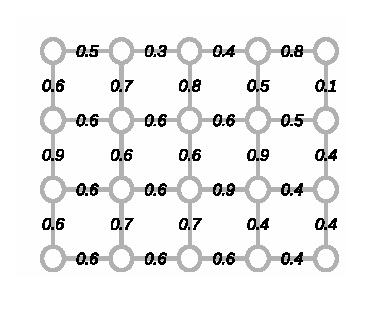
\includegraphics[scale=0.5]{Figures/affinity_graph}}\subfloat[]{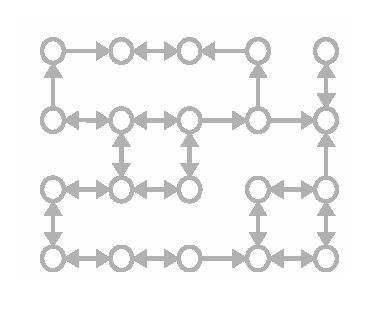
\includegraphics[scale=0.5]{Figures/sd_graph}}\subfloat[]{\includegraphics[scale=0.5]{Figures/sd_graph_plateaus}}\subfloat[]{\includegraphics[scale=0.5]{Figures/ws_result}}\protect\caption{(a) An disaffinity graph; (b) derived steepest descent graph; (c)
locally minimal plateaus (black), non-minimal plateau (gray), saddle
vertex (S), plateau corners (C); (d) the two basins of attractions
and border vertices (gray)}
\end{figure}


\textbf{Assigning border vertices. }In Fig. 1(d) we show the \emph{basins
of attraction} of the two \emph{regional minima.} The \emph{border}
vertices are shown in gray and belong to both \emph{basins of attraction.
}Watershed cuts \cite{Cousty2009,Cousty2010} assign \emph{border}
vertices with a single constraint that all the \emph{basins of attraction}
have to be connected. We introduce additional constrains. The watershed
transform has to be uniquely defined and the \emph{non-minimal plateaus
}should be divided evenly\emph{. }More specifically, we want our dynamics\emph{
}to be uniquely defined at \emph{saddle vertices, and }the vertices
of the \emph{non-minimal plateaus} to be assigned to the same \emph{basin
of attraction} as the nearest \emph{plateau corner - }a \emph{plateau
corner} reachable in fewest steps following the rules of our dynamics\emph{. }

\begin{figure}
\subfloat[]{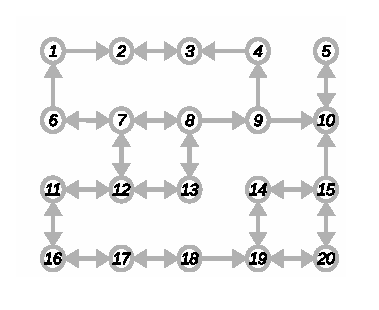
\includegraphics[scale=0.5]{Figures/sd_graph_ordered}}\subfloat[]{\includegraphics[scale=0.5]{Figures/sd_graph_plateaus_ordered}}\subfloat[]{\includegraphics[scale=0.5]{Figures/sd_graph_plateaus_modified}}\subfloat[]{\includegraphics[scale=0.5]{Figures/final_segmentation}}\protect\caption{(a) Vertex indices; (b) distances to the nearest plateau corner; (c)
modifications to the steepest descent graph; (d) final watershed partition
of the graph}
\end{figure}


\textbf{Watershed transform algorithm. }We introduce an ordering function
$\alpha:V\to\{1,2,...,|V|\}$ such that $\alpha(u)\neq\alpha(v)$
if and only if $u\neq v$. We'll refer to $\alpha(u)$ as the index
of $u$ (Fig. 2(a)). In the first part of the algorithm we modify
$D$ by removing edges. For all \emph{saddle vertices} we keep only
one outgoing edge - the one pointing to a vertex with the lowest index.
We then divide the \emph{non-minimal plateaus}. We initialize a global
FIFO queue $Q$. We then mark all the \emph{plateau corner} vertices
as visited and insert them into $Q$ in increasing order of their
index. While $Q$ is not empty we remove the vertex $v$ from the
top of the queue, we then follow all the bidirectional edges. If the
vertex $u$ on the other side of the edge is not visited, we mark
it as such, insert it to the back of the queue and change the edge
to be incoming. Otherwise, if the vertex was already visited we just
remove the edge. The resulting steepest descent graph is shown on
Fig. 2(c) - the dotted edges are removed. The connected components
of the modified \emph{descent graph $D$}, now considering all the
remaining edges as bidirectional will be our \emph{basins of attraction}.

The algorithm runs in linear time with respect to the number of edges
in $G$ and produces an optimal partitioning as defined in \cite{Cousty2009}.
The total number of segments in the partitioning will equal to the
total number of \emph{regional minima. }We defer the detailed algorithm
listing, the proof of correctness and running time analysis to the
supplementary material.

\textbf{Reducing over-segmentation}. Often the edge weights of $G$
represent \emph{disaffinities} - confidence that the two vertices
don't belong to the same segment. The \emph{disaffinity }between two
vertices not connected by an edge is considered to be infinite. The
\emph{saliency }of two adjacent segments is the value of the minimal
\emph{disaffinity} between the vertices of the two segments. Noisy
values of \emph{disaffinities }can produce severe over-segmentation
(Fig. 3(c)). In order to reduce the over-segmentation we often merge
adjacent segments with the \emph{saliency }below some given threshold
$T_{\min}$ \cite{Najman1996}. We are confident that \emph{disaffinities
}below $T_{\min}$ should yield connected vertices. An equivalent
segmentation can be obtained by replacing the weights of all edges
in $G$ with the weight smaller than $T_{\min}$ to a common low value
(e.g. $0$) before applying the watershed transform. We prove this
claim in the supplementary material. To show confidence about high
values of \emph{disaffinities}, and in order to prevent undesired
mergers, we introduce a threshold $T_{\max}$ by erasing all the edges
from $G$ with the weight higher than $T_{\max}$, and essentially
setting them to $\infty$. The $T_{\max}$ threshold can produce singleton
vertices in $G$. The singleton vertices are not assigned to any \emph{basin
of attraction} and are considered background, which is often a desired
result.


\section{Hierarchical Clustering of the Watershed Basin Graph}

A hierarchical clustering of an undirected weighted graph treats each
vertex as a singleton cluster and successively merges clusters connected
by an edge in the graph. A cluster is always a connected subset of
the graph's vertices. Each merge operations creates a new level of
the hierarchy - a flat segmentation where each cluster represents
a segment. In \emph{single linkage} clustering, each step we merges
two clusters connected by an edge with the lowest weight in the original
graph. \emph{Single linkage }clustering is equivalent to finding the
minimum spanning tree of the graph \cite{Gower1969}.

In this section we propose a size-dependent single linkage clustering.
The method can be applied to any edge weighted graph, however we find
it superior when used on the \emph{watershed basin graph} defined
as follows. Let $V_{W}=\{B_{1},B_{2},\dots\}$ be the set of \emph{watershed
basins} obtained by the watershed transform of a graph $G=(V,E)$.
We define the watershed basin graph of $G$ as $G_{W}=(V_{W},E_{W})$
where an edge $\{B_{i},B_{j}\}$ exists in $E_{W}$ for all neighboring
basins $B_{i}$ and $B_{j}$, and has the weight $w(\{B_{i},B_{j}\})$
equal to the \emph{saliency} of the two \emph{basins.} We will refer
to the vertices of the \emph{watershed basin graph} as \emph{basins}
and to the edge weights as \emph{saliencies.}

In our size-dependent \emph{single linkage} clustering method, in
each step we merge clusters with the lowest \emph{saliency} that don't
satisfy a given predicate. \emph{Saliency }of two clusters is defined
as the minimal \emph{saliency }of any two members:

\begin{equation}
d_{C_{1},C_{2}}=\underset{B_{i}\in C_{1},B_{j}\in C_{2},\{B_{i},B_{j}\}\in E_{W}}{\min}w(\{B_{i},B_{j}\})
\end{equation}


At the last level of the hierarchy all pairs of clusters will satisfy
the predicate.

\textbf{Size-dependent comparison predicate. }We define a predicate
$\Lambda,$ for evaluating whether two clusters should be merged.
The predicate is based on the sizes of the two clusters. Let $S(C)$
represent the size of $C$ (e.g. number of \emph{basins} in the cluster
or the sum of the \emph{basin }sizes). The size can be any measure
of a cluster with the property that $S(C_{1}\cup C_{2})\ge S(C_{1})$.
We first define a non-increasing threshold function of cluster size
$\tau(s)$. For a given cluster size $s$ the value $\tau(s)$ represents
the maximal \emph{saliency} allowed between a cluster of size $s$
and any adjacent cluster. Our predicate is then defined as:

\begin{equation}
\Lambda(C_{1},C_{2})=\begin{cases}
\textrm{t\textrm{rue}} & \textrm{if }d_{C_{1},C_{2}}\ge\tau\left(\min\left\{ S(C_{1}),S(C_{2})\right\} \right)\\
\textrm{false} & \textrm{otherwise\textrm{ }}
\end{cases}
\end{equation}


The intuition behind the predicate is to apply prior knowledge about
the sizes of the true segments. With the threshold function we control
the confidence required to grow a cluster of a certain size.

With a slight modification of the predicate we could allow for an
arbitrary threshold function (changing the condition to $d_{C_{1},C_{2}}\ge\min\left\{ \tau(S(C_{1})),\tau(S(C_{2}))\right\} )$.
However, restricting the function to be non-decreasing allows us to
design a more efficient\emph{ }algorithm. It is also more intuitive
to allow higher \emph{saliency} for merging small clusters and require
lower \emph{saliency} as the sizes of the clusters grow. As $\tau$
is required to be non-decreasing, we can rewrite the condition in
(2) as $\tau^{-1}(d_{C_{1},C_{2}})\ge\min\left\{ S(C_{1}),S(C_{2})\right\} $
allowing us to specify either $\tau$ or $\tau^{-1}.$ When $\tau^{-1}$
is constant the algorithm will tend to

\textbf{Algorithm 1 }In our clustering algorithm we visit all the
edges of the watershed basin graph in non-decreasing order and merge
the corresponding clusters based on the introduced predicate.
\begin{enumerate}
\item Sort $E_{W}$ into $\pi(e_{1},\dots,e_{n})$, by non-decreasing edge
weight.
\item Start with basins as singleton clusters $S^{0}=\{C_{1}=\{B_{1}\},C_{2}=\{B_{2}\},\dots\}$
\item Repeat step $4$ for $k=1,\dots,n$
\item Construct $S^{k}$ from $S^{k-1}$. Let $e_{k}=\{B_{i},B_{j}\}$ be
the $k$-th edge in the ordering. Let $C_{i}^{k-1}$ and $C_{j}^{k-1}$
be components of $S^{k-1}$ containing $B_{i}$ and $B_{j}$. If $C_{i}^{k-1}\neq C_{j}^{k-1}$
and $\Lambda(C_{i}^{k-1},C_{j}^{k-1})$ then $S^{k}$ is created from
$S^{k-1}$ by merging $C_{i}^{k-1}$ and $C_{j}^{k-1}$, otherwise
$S^{k}=S^{k-1}.$
\item Return the hierarchical segmentation $(S^{0},\dots,S^{n})$
\end{enumerate}
\textbf{Theorem 1 }\emph{The highest level of the hierarchical segmentation
produced by algorithm (1) will have the predicate $\Lambda$ satisfied
for all pairs of the clusters. The complexity of the algorithm is
$\left|E_{W}\right|\log\left|E_{W}\right|$. The algorithm can be
modified to consider only the edges of the minimum cost spanning tree
of $G_{W}$.}

We defer the proof the supplementary material.

The steps 2-5 of the algorithm have near linear complexity. Once we
have a sorted list of the edges we can re-run the algorithm for different
threshold functions more efficiently.

\begin{figure}
\subfloat[\label{fig:1a}]{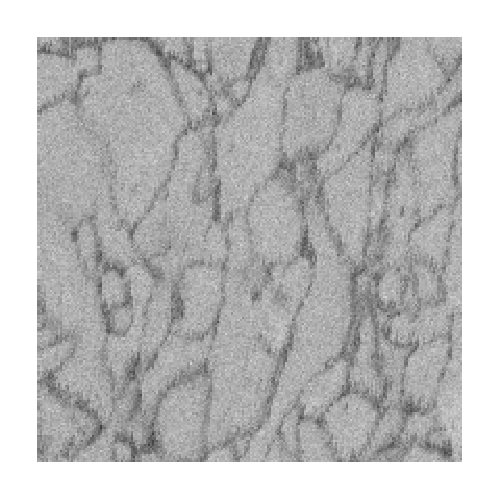
\includegraphics[width=3cm]{Figures/chan}}\subfloat[]{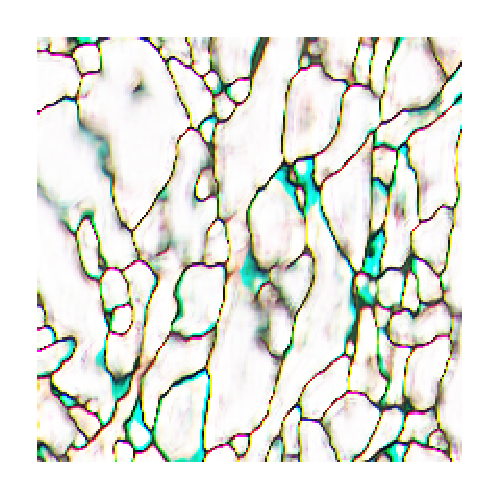
\includegraphics[width=3cm]{Figures/aff}}\subfloat[]{
\includegraphics[width=3cm]{Figures/raw}}\subfloat[]{
\includegraphics[width=3cm]{Figures/minmax}}

\subfloat[]{
\includegraphics[width=3cm]{Figures/gt}}\subfloat[]{
\includegraphics[width=3cm]{Figures/all}}\subfloat[]{
\includegraphics[width=3cm]{Figures/fe1}}\subfloat[]{
\includegraphics[width=3cm]{Figures/fe2}}\protect\caption{(a) EM image; (b) volumetric disaffinity graph, the 3 directions of
disaffinities are represented with RGB; (c) watershed transform output;
(d) watershed transform output with $T_{\min}=0.01$ and $T_{\max}=0.9$;
(e) ground truth; (f) our method; (g), (h) segmentation by \emph{\cite{Felzenszwalb2004}
}with $k=0.5$ and $k=10$ respectivelly.}
\end{figure}





\section{Results}

We have applied our method to 3D electron microscopic (cite e2198)
brain images (Fig. 3(a)). We obtained disaffinity graphs with values
in $\left[0,1\right]$ range using convolutional neural networks described
by Turaga \emph{et al.} \cite{Turaga2009,Turaga2010} (Fig. 3(b)).
We define the size of a segment to be the number of 3D pixels contained
inside the segment. In the first step we have applied our watershed
transform with thresholds $T_{\min}=0.01$ and $T_{\max}=0.9$. We
have tested our method on three intuitive threshold functions. The
first one enforces all the segments to be at least some size, second
and the third one require the minimal size of the segment to be proportional
to the affinity (square of affinity) and are therefore allowing bigger
object to be created....

\begin{figure}
\subfloat[]{\includegraphics[width=7cm]{Figures/results}}\subfloat[]{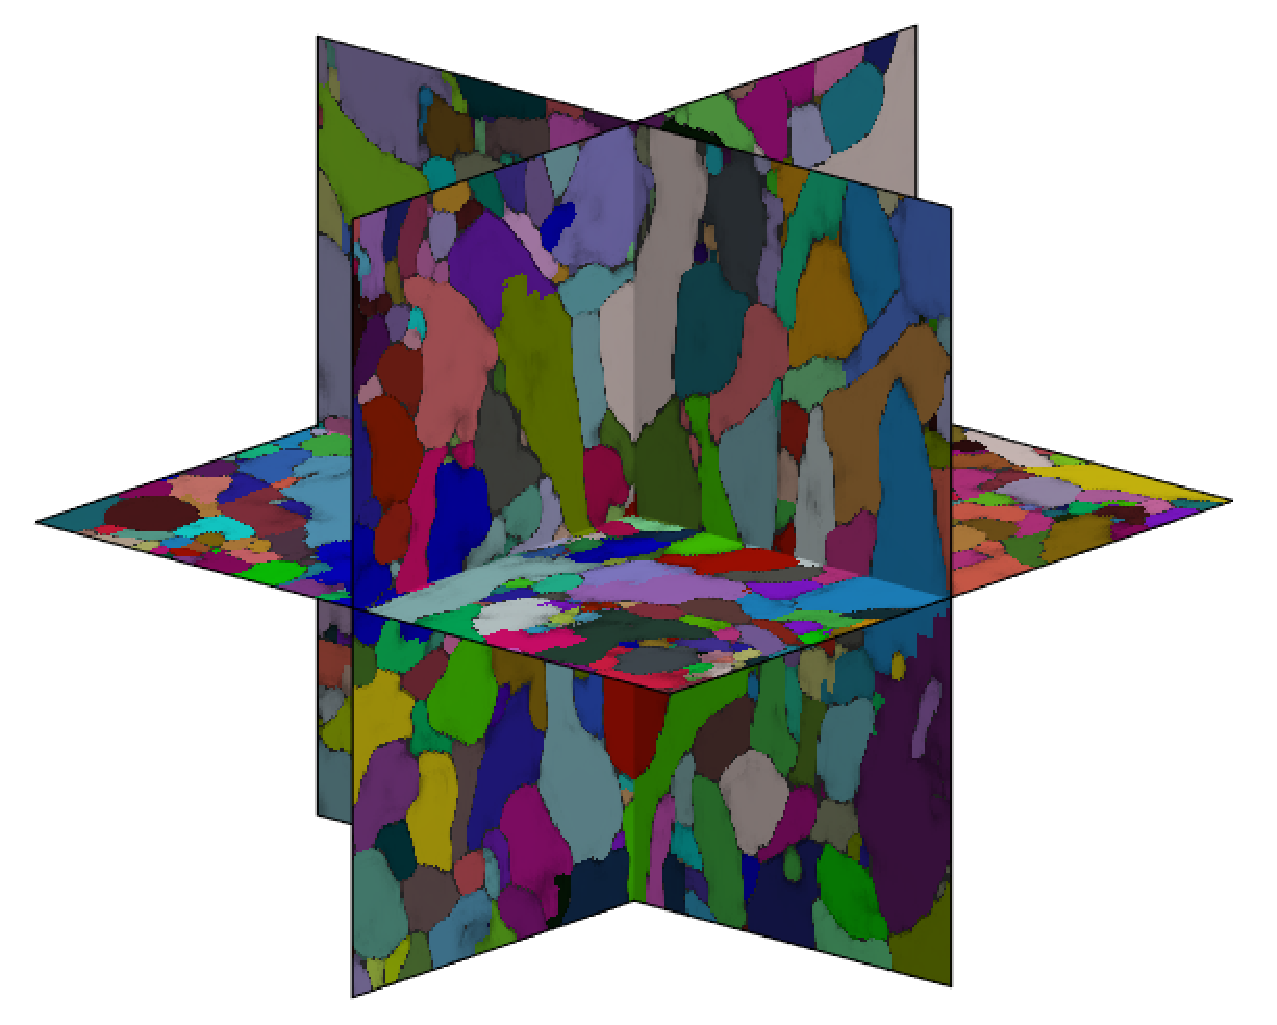
\includegraphics[width=5.5cm]{Figures/3da}}\protect\caption{(a) Performance of our method and the method described in \cite{Felzenszwalb2004};
(b) Segmentation obtained by our method with $\tau^{-1}(w)=1000(1-w)$}
\end{figure}



\subsubsection{Metric}

A good metric for evaluating a segmentation should ideally tell us
how good the segmentation is for using in practice. Mainly how much
manual corrections are needed to acheve the correct segmentation.
Often foreground-restricted Rand Index \cite{Rand2009} between the
proposed segmentation and the ground truth is used. However it has
problems when the number of segments is large as the dynamics range
gets smaller. A better metric is introduced by introduced by Arganda
at al, separating the rand indices for splits and mergers. Explain
the metric briefly.

We see that the method blah starts introducing mergers for some values
of k while there's still a lot of splits around. It's because the
other method has stricter guarantees (not to corse or fine) where
as we we relax the too corse requirement and just hierustically produce
a segmentation that is not too fine. (not sure we need this)


\section{Conclusions}

Our method is superior for segmenting images where we have prior knowledge
about the size of the true segments, which makes it ideal for segmenting
3D EM images. For conservative threshold functions our method can
greatly reduce the number of segments without introducing mergers,
which makes it ideal as pre processing method for some other methods.
Final segmentation can be obtained by merging our segments. It would
be a good input to a lot of other methods like \cite{Mustafa}prior
knowledge about segments assumes all have the same size properties


\renewcommand\bibname{References}

\bibliographystyle{splncsnat}
\bibliography{References/references}

\end{document}
